\chapter{Alignment with Tandem Repeats} \label{CHAPTER:REP}
\todo{Prikla. Bud tu alebo do celkoveho intra}

A \firstUseOf{Tandem repeat} is a region in the genomic sequence that contains
two or more consecutive repetitions of some \firstUseOf{motif}, which is a
short genomic sequence. The instances of the motif in a tandem repeat are
called \firstUseOf{repetitions}.  Tandem repeats, like other sequences, undergo
evolution, and therefore events like mutations, insertions, and deletions
occurs in the individual repetitions.  Therefore individual repetitions are
only approximate copies of a motif.  More than $2\%$ of the human genome is
covered by short tandem repeats, and they occur in many genes and regulatory
regions \cite{Gemayel2010}. Additionally, recent short insertions in the human
genome are mostly caused by tandem duplication \cite{Messer2007}. Most of the
tandem repeats have evolved by tandem segmental duplications, which means that
a tandem repeat was created by several successive duplication events. The
consequence is that the homologous tandem repeats in two related sequences can
contain a different number of copies of the original motif. Note that it is
possible that none of the current repetition is the exact copy of the original
motif.

Aligning homologous tandem repeats is hard, because it is not clear which
repetitions are orthologous (which originate in the same ancestral repetition).
Tandem repeats do not only affect quality of alignment within them, but the
error can spread into adjacent columns of an alignment, as we show in Section
\ref{SECTION:REPSIMRESULTS}, Figure \ref{FIGURE:SFF_GRAPHS}.  These
inaccuracies can spread further and cause artifacts in the results of
comparative genomic methods that use sequence alignments.

In this chapter, we introduce a tractable model that explicitly accounts for
tandem repeats. We use the maximum expected gain framework to explore several
decoding criteria for our model. We evaluate our model using simulated data.
Evaluating model on real data is hard, because we do not know the correct
annotation of the real DNA sequences and we have to use indirect methods for
evaluation. We do not present such comparison in this thesis, but such
comparison can be found in \cite{Nanasi2014}.

\section{Related work}\label{SECTION:REPALNMETHODS}

\todo{vysvetli jasnejsie. Naskor problem, potom alg, k algoritmu netreba
detaily, len zlozitost} Alignment methods that take into consideration tandem
duplications were first studied by Benson \cite{Benson1997}, who proposed
extension of the Needleman-Wunsch algorithm. In their scoring scheme, they
scored duplications as a separate event. Each duplication was penalized by the
duplication initiation cost, the duplication extension costs for each
repetition and Needleman-Wunsch like scoring scheme to score original string
with its repetitions. Time complexity of this algorithm is $O(n^4)$, and Benson
also proposed a heuristic algorithm to compute the alignment in a reasonable
time.  Several variants of this problem were also studied \cite{Sammeth2006,
Berard2006, Freschi2012}\todo{Pripadne spomen v com sa lisia}. It is also
possible to use a lossy compression scheme to collapse tandem repeats, and then
align compressed sequences \cite{Freschi2012}.

A Traditional approach to deal with tandem repeats is to mask them in both
sequences and then align masked sequences by some alignment algorithm.  Masking
means replacing tandem repeats and other low complexity regions either with
lower-case letters (soft-masking) or with N symbols (hard-masking, N represents
any base). Masking is done by some method for finding tandem repeats, such as
\abbreviation{Tandem Repeat Finder}{TRF} \cite{Benson1999}, TANTAN
\cite{Frith2011}, mreps \cite{Kolpakov2003}, or ATRhunter \cite{Wexler2005}. 

Methods mentioned above were not based on probabilistic models. The first
probabilistic method specifically targeting tandem repeats was introduced by
Hickey and Blanchette \cite{Hickey2011}.  They developed a context-sensitive
model based on pair Tree-Adjoining grammars.  Their model does not explicitly
model an arbitrary number of repeats; it focuses on short context-sensitive
indels caused by tandem duplications, because majority of short indels are
caused by tandem duplication ($90\%$ \cite{Hickey2011}). The time complexity of
their decoding algorithm is $O(n^2L^2)$, where $n$ is the length of the
sequences and $L$ is the maximal length of context sensitive indels.\todo{mozno
trochu napi co ich model robi (nie presne ako)}

Another, partially probabilistic method was developed by Kováč {\it et al.
(2012)}\nocite{Kovac2012}. The aim of the method was to align repetitive motifs
occuring in some protein families (for example zinc finger proteins), which are
similar to tandem repeats in DNA. Their method focused on correctly aligning
individual occurrences of the motifs. They combined a profile HMM of the motif
and a pair HMM, and developed a new decoding algorithm similar to the Viterbi
algorithm. Despite the use of probabilistic models, their method was not a
probabilistic model, because scores from different models were combined in an
ad-hoc manner. 

Hudek \cite{Hudek2010} developed an algorithm which combines of the Viterbi and
posterior decoding. The goal of the algorithm was to reduce misalignments due
to short tandem repeats with the motif length $1$, for example $AA$ in the
first sequence and $AAAAAAAAA$ in the second sequence. The algorithm developed
by Hudek considers all possible alignments of $u$ and $v$\todo{co su u a v} in
the final alignment. The algorithm segments the alignment into blocks, such
that each block contain gaps in only one sequence. They developed pHMM model
that defines probability distribution over all possible segmentation of
alignments of input sequences and give the algorithm that finds the most
probable segmentation.  Unlike Viterbi algorithm, their algorithm considers all
possible alignments within each segment.\todo{strasny chaos}

\section{Finding Tandem Repeats}
Although our main goal is to align sequences with tandem repeats, our model
will feature submodels that can be used to find the repeats in a single
sequence. In this section, we describe our repeat submodel and repeat model
from the TANTAN repeat finder \cite{Frith2011}. We start by describing
non-probabilistic approach to finding repeats, which we also use in the
preprocessing phase of our method.

\subsection{Tandem Repeat Finder}

Probably the most popular method for finding tandem repeats is the Tandem
Repeat Finder (TRF) \cite{Benson1999}.  Tandem repeat finder finds the position
of a tandem repeat (referred as an \firstUseOf{interval}), consensus sequence
(an approximation of the original motif), alignment of the consensus sequence
and the input sequence, and various other information about each repeat.

The method consists of two components: detection and analysis. The detection
component tries to find a set of candidate tandem repeats by analyzing the
distances between occurrences of the same $k$-tuple (substring of length $k$).
It uses several statistical criteria to detect repeats and distinguish between
tandem repeats and non-tandem repeats \cite{Benson1999}.

The analysis component aligns a candidate consensus using wraparound dynamic
programming \cite{Myers1989} with the surrounding sequence. If the alignment is
not successful (candidate consensus has to be aligned at least twice to be
successful), candidate repeat is discarded. Otherwise, the final consensus
sequence is computed from the alignment along with other statistics about
tandem repeat.

Tandem repeats found by the TRF are often redundant.  They can overlap, have slightly
different consensus motifs, the motifs can be shifted cyclically, and can have
different lengths, as in the following example:

\begin{verbatim}
Sequence  X:        CACCGCCACCACCGTAG
Consensus ACCACC:    ACCACCACCACC      2 repetitions
Consensus AAC:       ACCACCACCACC      4 repetitions
consensus CAC:      CACCACCACCACC      4.3 repetitions
\end{verbatim}

The sequence $X$ contains a tandem repeat and there are three consensus
sequences with different number of repetitions. Note that the repetition of the
consensus can be incomplete; as with the $CAC$ consensus where we have $4.3$
repetitions ($0.3$ stands for the last $C$ in the repetitive sequence).  Note
that the purpose of this example to illustrate possible redundancies in the TRF
output.  If we actually run TRF on sequence $X$, the output would be only the
repeat with consensus $CAC$.

\subsection{Sunflower Model}\label{SECTION:SUNFLOWERMODEL}
The \firstUseOf{sunflower model} is an HMM that represents tandem repetious of
one previously specified motif $C=c_0\dots c_{k-1}$. We have developed this
model as a part of our model for aligning sequences with tandem repeats, which
we describe in section \ref{SECTION:REPMODELS}, but it can be also used as a
simple tool for finding tandem repeats and we use it to improve a candidate set
of tandem repeats initially constructed by the TRF program (see Section
\ref{SECTION:REPOPT}).

The sunflower model is an extension of the profile HMM described in Section
\ref{HERD:METHODS} (see Figure \ref{FIGURE:PROFILEHMM} on page
\pageref{FIGURE:PROFILEHMM}). In particular, the sunflower model is a circular
version of the profile HMM with match states representing motif $C$. This model
implicitly assumes that repetitions evolved from motif $C$ independently of
each other, as of at single point of time, motif $C$ was copied several times
forming tandem repeat, which then underwent several simple evolution events (
substitutions, deletions and insertions). This does not accurately reflect a
typical evolution history of a tandem repeat, where individual repetitions
arise over time from existing copies which could differ from the original
consensus $C$. However, trying to model such evolution would lead to a much
more complicated model.

\begin{figure}
\begin{center}
\begin{subfigure}[b]{0.5\textwidth}
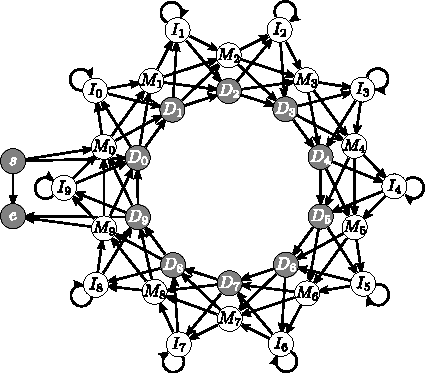
\includegraphics{../figures/SunflowerSilentCircle.pdf}
\caption{Cyclic profile model}\label{SUBFIGURE:SUNFLOWERSILENTCYCLE}
\end{subfigure}%
\begin{subfigure}[b]{0.5\textwidth}
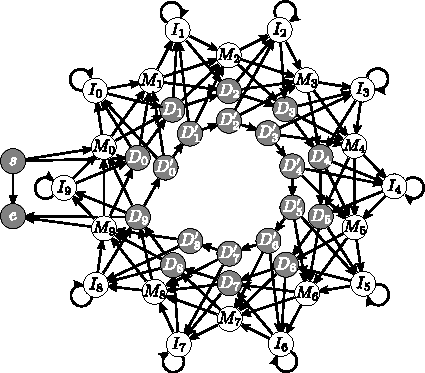
\includegraphics{../figures/Sunflower.pdf}
\caption{Sunflower model}\label{SUBFIGURE:SUNFLOWER}
\end{subfigure}
\end{center}
\caption[Example of the Sunflower model]{Example of the Sunflower model 
with the motif of length $10$. White states emit one character and gray states are
silent states. States $s$ and $e$ are initial and final silent states. Sunflower model
has additional delete states $D'_0, \dots D'_8$ to remove silent cycle from the
model.}
\label{FIGURE:SUNFLOWERMODEL}
\end{figure}

Our model contains typical profile HMM states $M_0,\dots, M_{k-1}, I_{0}, \dots, I_{k-1}$
and $D_{0}, \dots, D_{k-1}$. The transitions between the states are similar to
profile HMM:  $M_{i}\to M_{i\oplus 1}, M_i\to I_i, M_i\to D_{i\oplus 1}, I_i\to
I_i, I_i\to M_{i\oplus 1}, I_i\to D_{i\oplus 1}, D_{i}\to D_{i \oplus 1},
D_{i}\to M_{i\oplus 1}, D_{i}\to I_i$ for all $0\leq i < k$, where $\oplus$ is
$+$ modulo $k$. As in the profile HMM, states $D_i$
are silent. We add silent start state $s$ and silent final state
$e$ with transitions $s\to M_0, s\to D_0, D_{k-1}\to e, M_{k-1}\to e$ and
transition $s\to e$ to model empty tandem repeats. The whole model topology is shown in
Figure \ref{SUBFIGURE:SUNFLOWERSILENTCYCLE}.

The problem is that the cyclic profile contains a cycle of silent states, which
causes problems with training and decoding algorithm (see Section
\ref{SECTION:SILENT}. Removing these states would lead to additional
$\theta(k^2)$ edges. Therefore, we have decided to remove
the transition between delete states $D_{k-1}$ and $D_0$. To compensate for the lost
possibility of deleting an arbitrary part of the tandem repeat, we add an
additional chain of delete states $D'_0, \dots, D'_{k-2}$, which are accessible
only from state $D_{k-1}$ by transition $D_{k-1}\to D'_0$, and their outgoing
transitions are similar to delete state transitions: $D'_{i}\to M_{i+1},
D'_{i}\to I_i$ for $0\leq i\leq k-2$ and $D'_{i} \to D'_{i+1}$ for $0\leq i <
k-2$. Note that $D'_{k-2}$ is connected only to $M_{k-1}$ to avoid passing a
full circle by delete states. The full model is in Figure
\ref{SUBFIGURE:SUNFLOWER}. We call this model the \firstUseOf{Sunflower} model.

This model has $4k+1$ states and $12k+1$ transitions, out of which $2k+1$
states are silent. There are $14k+2$ parameters to train for a motif $C$
(including emissions of insert and match states over the alphabet if size $4$).
Models with such a large number of parameters are hard to train, so we reduced
the number of parameters as follows. First, we tied similar transitions, so
that they have the same probability.  We used the set of parameters $p_{ab}$
where $a,b\in \{m, i, d, \cdot\}$, where $m$ stands for any match state, $i$
stands for any insert state, $d$ states for any delete state (from both
chains), and $\cdot$ is either start or final state. Therefore the probability
of transition from match state to delete state is $p_{md}$ and probability of
transition from insert state to final state is $p_{i\cdot}$.  Probabilities
were set so that $\sum_{b\in\{m,i,d\} p_{ab}}=1$ for all possible $a$.
Therefore, transitions from states $M_{k-1}, D_{k-1}$ and $D'_{k-1}$ do not sum
to $1$, because they are either missing one transition or having one additional
transition. For those states, the probability of transitions were normalized in
order to form a probability distribution. 

To reduce the number of emission parameters, all insert states share the same
emission distribution. For the emission distribution of match state $M_i$ we
assumed that the consensus base $c_i$ from the motif evolved over evolutionary
time $t$ according to Jukes-Cantor model\footnote{ The parameter $t$ of
Jukes-Cantor model is not time as measured by years, but rather a branch length
in an evolutionary tree obtained by multiplying of substitution rate and time.
More details can be found in \cite{Durbin1998}.  }. Jukes-Cantor model is a
theoretical model of evolution that assumes constant rate of evolution. Under
this model base $B_1$ evolved over time $t$ to different base $B_2$  with
probability $1/4(1-\exp(-4t/3))$.  The probability that $B_1$ after time $t$
will be still (or again) $B_1$  is $1/4(1+3\exp(-4t/3))$ \cite{Durbin1998}.
Time $t$ was the same for all match states. Therefore emissions of all states
are specified using only $4$ parameters ($1$ for match states and $3$ for
insert states).

To use the sunflower model models for finding tandem repeats, we have to add
state $B$ that models non-repetitive part of the sequence. Let $S_C$ be the
sunflower model for motif $C$. We add the transitions from $B$ to the start
state of $S_C$ and from the final state of $S_C$ to the state $B$. The
probability of transition from the state $B$ to the submodel $S_C$ is $p_r$,
the probability of repeat starting at particular position in the sequence.
Probability of transition from final state of $S_C$ to $B$ is $1$.  There is
also transition $B\to B$ with probability $1-p_r$. We can use the Viterbi
algorithm with this model to find all occurrences of tandem a repeat with motif
$C$. However, with this model we can search only for a specific motif. We call
this method of finding tandem repeats the \abbreviation{Sunflower repeat
finder}{SRF}.

\subsection{TANTAN}\label{SECTION:TANTAN}

\firstUseOf{TANTAN} is a high-order HMM aimed at finding tandem repeat
developed by Frith \cite{Frith2011}. Unlike the Sunflower model, TANTAN models
tandem repeats with an arbitrary motif. Its only restriction is the maximal
length of the motif $K$. In this section, we describe the core of the model;
the part that models tandem repeats. This core can be transformed to the model
usable for search by adding a background state $B$ as we described for the
Sunflower model.

\begin{figure}
\begin{center}
\begin{subfigure}{0.19\textwidth}
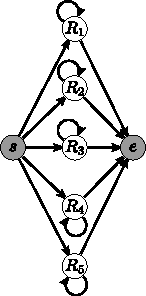
\includegraphics{../figures/tantan_simple.pdf}
\caption{Simple model}\label{FIGURE:TANTAN:SIMPLE}
\end{subfigure}%
\begin{subfigure}{0.3\textwidth}
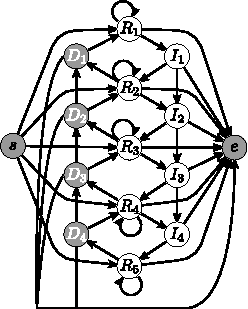
\includegraphics{../figures/tantan_indel.pdf}
\caption{With indels}\label{FIGURE:TANTAN:INDEL}
\end{subfigure}%
\begin{subfigure}{0.35\textwidth}
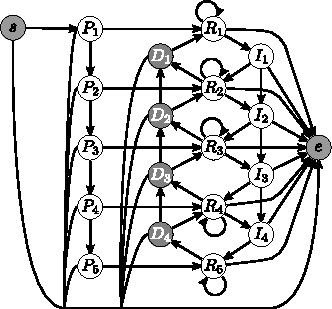
\includegraphics{../figures/tantan_init.pdf}
\caption{With first repetition}\label{FIGURE:TANTAN:INIT}
\end{subfigure}%
\end{center}
\caption{Three variants of the core of the TANTAN model. Gray states are
silent. The first one is a simplified model, only containing repeat states. The second
was used by Frith \cite{Frith2011}, allowing insertions and deletions.  The last one
is our extension with additional prefix states $P_1, \dots P_K$ which model
the first repetition.}\label{FIGURE:TANTAN}
\end{figure}

The principal idea is to use the state of order $l$ to model a repeat with
motif length $l$. TANTANs high order states uses less information than standard
high order states. Emission of symbol $X[i]$ in a standard state of order $l$
depends on subsequence $X[i-l:i]$.  Emission in TANTANs states of order $l$
depends only on the symbol $X[i-l]$. The model consists of $K$ high-order
states $R_l$, $1\leq l\leq K$ called repeat states, where state $R_l$ is of
order $l$. Emission of state $R_l$ is set so that the state emits the same
symbol as $X[i-l]$ with a high probability. By adding transition $R_l\to R_l$
we obtain an HMM modeling tandem repeats without indels with a motif of length
$l$. By connecting states $R_1,\dots, R_K$ to a single start and final state as
shown in Figure \ref{FIGURE:TANTAN:SIMPLE}, we obtain an HMM that models
repeats with the motif lengths $1$ through $K$.

This simplified model does not allow insertions and deletions in repetitions.
Indels are handled similarly to a profile HMMs, by adding insert states
$I_1,\dots, I_{K-1}$ and silent delete states $D_1, \dots, D_{K-1}$ connected
as in the Figure \ref{FIGURE:TANTAN:INDEL}. There are however significant
differences from profile HMMs.  In a profile HMM, delete states are used to
skip at least one match state, while in TANTAN a delete state is used move to a
state with a lower order. Conversely, insert states allows us to move in the
opposite direction; using insert state causes an increase of the order of the
repeat state.  It is also possible to move from the insert state $I_{j}$ to the
insert state $I_{j+1}$, which is not possible in a profile HMM.

One disadvantage of the TANTAN model is that it does not model the first
occurrence of the motif sequence, since repeat states model only the
subsequence repetitions of the sequence. This caused problems when we wanted to
incorporate TANTAN as a submodel for aligning sequences. Therefore we have
added an additional chain of prefix states $P_1,\dots, P_K$ modeling the first
repetition. Transitions from the start state are now only to the final state
(modeling an empty sequence) and the state $P_1$. State $P_l, 1\leq l\leq K$
has transitions to the final state, repeat state $R_l$ and the state $P_{l+1}$,
if such a state exists.

%Emisie a sme hotovy
We set emission distribution of the insert and prefix states to the background
probability: the distribution of the bases in DNA. Emission state of the state
$R_l$ was derived using Jukes-Cantor model with parameter $t$, where the
emission $X[i]$ evolved from $X[i-l]$ over time $t$.

\todo{Napis nieco o predpokladoch tohto modelu, porovnas so Sunflower}

\section{Models for Aligning with Tandem Repeats}\label{SECTION:REPMODELS}

In this section we describe models that we have designed and used in our
methods. We describe the model in an dual way; as a generalized pHMM and as an
equivalent non-generalized pHMM (emissions length is at most $1$ in both
sequences). The distribution of generated alignments and annotations (with
certain annotation functions) are same in both models, but clearly the
distribution of state paths will be different due to different sets of states.

The generalized model is obtained by taking the simple 3-state pHMM model from section
\ref{SECTION:ALIGNWITHPHMM} and adding a single generalized pair state $R$,
called the \firstUseOf{repeat state}, which in a single step generates tandem
repeats in both sequences. \reformulate{State $R$ can in theory generate
arbitrary long sequences which does not produce an alignment of tandem repeats
during decoding. Its task is to filter out tandem repeats of alignment, so that
they do not cause biases in the parts of an alignment emitted by other states
(match and indel states). We align homologous tandem repeats later in a
post-processing step.}{trochu tu miesas generovanie a decoding. mozno by som
toto presunula dalej, ked bude jasnejsie ako model vyzera. Skus na s 86} The
overall topology of GpHMM is illustrated in the Figure
\ref{FIGURE:REPEAT_GENERAL}.

To made this model more flexible, the emission distribution of state $R$ is
defined by an additional pHMM. Since the repetitions in the tandem repeat are
very similar to each other, we did not try to model the evolution of repetitive
parts of the sequences. We assumed that repeat evolved from the original motif
by one event, and then repetitions evolved independently. The goal of state $R$
is to model such evolution in single generalized emission. Model was
constructed from the Sunflower models. Let $C$ be the set of all motifs that
can occur in the alignment. For each motif $c\in C$ we created sunflowers
$S_c^X$ and $S_c^Y$.  Sunflower $S_c^X$ is the sunflower model with motif $c$
which generates symbols only in sequence $X$; $S_c^Y$ generates symbols in $Y$.
We connect $S_c^Y$ and $S_c^X$ by a transition from the final state of $S_c^X$
to the start state of $S_c^Y$ with probability $1$ and thus getting model $H_c$
that generates repeats in both sequences. We connected models $H_c$ for all
$c\in C$ in parallel by a single start state and a single final state as in
Figure \ref{FIGURE:REPEAT_GENERAL}. The probability of the transition from the
start state of $R$ to the start state of model $H_c$ was proportional to the
distribution of motifs $\prob{c}$. Note that the size of this model is
determined mostly by the total length of all motifs, and therefore this model
can be very large, even infinite if we consider all possible sequences as
possible motifs for tandem repeats.  To keep the model size reasonable, we
computed a set of candidate motifs $C$ and use it for construction of the
model. More details are in section \ref{SECTION:REPOPT}. We call this
generalized model the \abbreviation{sunflower field}{SFF} model.

\begin{figure}
\begin{center}
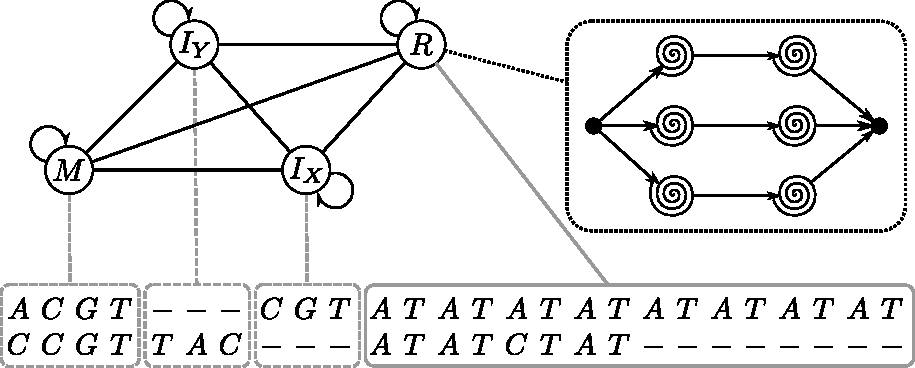
\includegraphics[width=14cm]{../figures/PairRepeatHMMGeneral.pdf}
\end{center}
\caption[General topology of Repeat pHMM]{ 
Topology of the Repeat pHMM. We extended the 3-state pHMM with one generalized
state $R$, which in one emission generates tandem repeats in both sequences.
The emission distribution of state $R$ is defined by another pHMM shown in a
dotted box (*). Bellow the model we show an example of emitted alignments.
Dashed gray lines corresponds to multiple emissions from the same states, while
the full line represents one emission from a generalized state. 

(*) Black states in this submodel silent start and final states. Spirals
represents sunflower submodels. They are in
pairs of two identical models $S_c^X$ and $S_c^Y$, one for generating tandem repeat in one
sequence, other for generating tandem repeat in the other sequence. There are
multiple pairs of submodels, each for modeling different motif $c$.
 }\label{FIGURE:REPEAT_GENERAL} 
\end{figure}

We also experimented with using a TANTAN-like model for defining emissions
distribution of state $R$. We used the TANTAN model with the prefix states from
Section \ref{SECTION:TANTAN}. Similarly as with the sunflower model, we created two
copies of TANTAN, each generating repeats in only one sequence and connect them
together exactly as we would connect the sunflower models. Since TANTAN model does
not rely on a motif, it is not necessary to create more copies of the TANTAN HMM and
its general topology looks like SFF's with only one motif.  Since TANTAN is
a high order HMM, the resulting model is a high order and generalized pair HMM.
We refer to this model as \abbreviation{TANTAN pHMM}{TTP}. The advantage of
this model over SFF is in it's size, since TTP will have in practice fewer
states than SFF. \todo{Povedz ze pri jednom zalezi od max dlzky, kym druhy od
suctu dlzok konsenzov} However, TTP models evolution of repetitions
differently, since each repetition is created from the previous repetition and
tandem repeats in sequences $X$ and $Y$ are independent of each other; there is
no penalty for them having different motifs.\todo{Nejaka dalsia diskusia o vlastnostiach modelov? Napri ** zo strany 84 a *** zo strany 87}

Both SFF and TTP are defined as $4$ state high order GpHMMs.  In general, using
generalized models increases the time complexity of decoding algorithms
quadratically. Therefore we also used expanded versions of the models: we
replaced the generalized state $R$ with the pHMM submodel defining emissions of
$R$. All transitions entering into $R$ were replaced by transitions to the
start state of the submodel, and all outgoing transitions from $R$ were
replaced by transitions starting in the final state of the submodel. This
transformation does not change the distribution of alignments generated by the
model.  Additionally, the distribution of alignment annotations does not
change, if we use the following annotation functions. \reformulate{For the
original GpHMM we can use the identity function as a labeling function
$\Lambda_{ID}$. For expanded model we then use function $\Lambda_R$, which
labels all states from submodel by label $R$ and other states by the same label
as in GpHMM. }{Toto nesedi s definiciou anotovaneho zarovnania na str 88,
radsej zmaz}

\paragraph{Parameter estimation:}
In our experiments, we have used $310,091$ consensuse sequences found by the
TRF program on the human chromozome 15 and its orthologous sequences in the dog
genome as motifs for building SFF.  The probability of choosing a particular
motif is the observed frequency of the motif in the TRF output. \reformulate{In
practice, we limit the Sunflower submodels only to those which was found by the
TRF in the input sequence.  Additionally, if the input sequence contain motif
that is not in the predefined set, we add it to the model with the probability
of the least occurring motif in the model.}{Mas v 4.5, tento text nie je prilis
jasny}

We set the parameters of the Sunflower submodel manually: the insert and delete
rates were set to $0.005$, the match states allows mutations from motif
sequence according to the Jukes-Cantor model with parameter $t=0.05$. The
emission of the insert states were set according to the frequency of the bases
in the input human-dog alignment.  Parameters of the TANTAN submodel were
estimated by the Baum-Welch algorithm \cite{Durbin1998} on 500 repeats sampled
from the SFF model.

\todo{Dva odstavce dole: preco tu? ***}
The size of the TTP model depends on the length of the longest possible motif,
which we set to $50$ bases. The size of the SFF model depends on the total
length of all motifs used. Therefore the SFF model can be exponentially larger than the TTP
model. The SFF model assumes that repetitions accumulated mutations
independently, while the TTP model assumes that each repetition evolve from the
previous occurrence of the repetition. Additionally, there is no dependence of
tandem repeats between the two sequences in the TTP model, while in the SFF
mode they use the same consensus.

Tandem repeats at orthologous positions in two species may share common
ancestor and therefore share part of their evolutionary history. However, it is
possible that they were consequently modified by additional evolution events
after speciation (including more tandem duplications). In our model, we ignore
such complex evolution of repetitions, because it would lead to very complex
model and increase the difficulty in decoding and training. Kováč {\it et. al}
developed a method with limited dependence by adding repeat submodels emitting
copies in the two sequences at same time \cite{Kovac2012}.

\todo{Ako si nastavil parametre 3-stavoveho model a pr. predchodu do R}

\section{Decoding methods}\label{SECTION:REPDECODING}

\todo{Preco sme to robili? Nejaky uvod? Mic: asi by som chcel spomenut luntera,
kde som to popisoval, ako aj nasu pracu a inych, ta preto sme chceli pouzit aj
rozne dekodovacie sposoby}

In this section we describe several optimization criteria that we used with
the 3-state model, the SFF model and the TTP model: the \abbreviation{Viterbi
algorithm}{VA}, the \abbreviation{posterior decoding}{PD}, the
\abbreviation{marginalized posterior decoding}{MPD}, the \abbreviation{block
Viterbi algorithm}{BVA} and the \abbreviation{block posterior decoding}{BPD}.
The first three methods are used with the non-generalized versions of the models, the latter
two methods (block methods) are used with GpHMMs. We
have already described the first three algorithms in Section
\ref{SECTION:ALNDECODING}. Here we introduce the highest expected gain framework
for pair HMMs and formulate all algorithms using gain functions.

In Section \ref{SECTION:HEG} we defined a gain function as a functions of two
annotations. For pair HMMs we define a gain function as a function of two
annotated alignments consisting of alignment columns along with annotation
symbols. This is necessary, because we use generalized models, and therefore
annotation symbols do not uniquely determine the alignment (there can be
multiple alignments with the same annotation).

We represent columns of an annotated alignment using indices to sequences and annotation
symbols. In the case of generalized models, which can generate more than one
column in one step, only the first column will contain annotation symbol, other
columns will contain symbol $\varnothing$. Formally, an \firstUseOf{annotated
alignment} of length $t$ of sequences $X=x_0x_1\dots x_{n-1}$ and
$Y=y_0y_2\dots y_{m-1}$ is represented as a sequence of tuples $(u_0, a_0,
b_0), \dots, (u_{t-1}, a_{t-1}, b_{t-1})$ where $a_i\in \{0, \dots,
{n-1}\}\cup\{-_0, \dots, -_n\}$ and $b_i \in \{0, \dots, m-1\}\cup\{-_0, \dots,
-_m\}$, and $u_i$ is either an annotation symbol or symbol $\varnothing$.
Number $i$ represents $i$-th symbol in the corresponding input sequence and
$-_i$ represents a gap in the sequence before position $i$ (if $i$ is the
length of the sequence, it represents the gap at the end of the sequence). For
example $(I_X, 47, -_{42})$ means that $x_{47}$ is aligned to a gap that is
between $y_{41}$ and $y_{42}$ and that this column has annotation $I_X$.
Naturally, indices in $a_i$ and $b_i$ have to be in non-decreasing order, and
each non-dashed symbol has to be in the corresponding sequence in the alignment
exactly once. Additionally, $a_0$ has to be $0$ or $-_{0}$, $a_t$ is $n$ or
$-_n$. The constrains for $b$ are analogous.  The first annotation symbol
$u_0\not=\varnothing$ and if some $u_i$ is equal to $\varnothing$ then such a
column was emitted by the same emission as the previous column.  If we use a
non-generalized model, the annotated alignment cannot contain symbol
$\varnothing$. The reason for using annotation symbol $\varnothing$ is that we
need to distinguish between different generalized emissions. We can define the
probability of an annotated alignment $\Lambda$ as the sum of the probabilities
of the state paths that generate such an alignment and \reformulate{the state
paths annotation is equal to the}{WTF?} annotation from $\Lambda$. We denote
this probability as $\prob{\Lambda\mid X, Y}$. We will refer to triple $(u_i,
a_i, v_i)$ as an \firstUseOf{annotated alignment column}.\todo{Toto chces dat
asi skor (asi mysli annotated alignment column}

We are interested in the \firstUseOf{repeat annotation} with annotation
function $\lambda_R$.  For generalized SFF and TTP (and 3-state pHMM),
$\lambda_R$ is the identify function. For the non-generalized versions,
$\lambda_R(u)=R$ for all states $u$ from the submodels modeling tandem repeats.
The probability of a \reformulate{state path}{to si asi definoval?} and
annotation is defined exactly as for HMMs that generate only one sequence.

Similarly as for the regular HMMs, we can define a gain function $G(\Lambda,
\Lambda')$ that corresponds to ``similarity'' of two annotated alignments
$\Lambda$ and $\Lambda'$. Note that for HMMs, symbol $\Lambda$ represents
annotation; with pHMMs, we use this symbol for an annotated alignment.  Since a
pHMM defines the probability distribution $\Lambda_T$ of the correct annotated
alignments, we can define the expected gain of an annotated alignment given
sequence $X$ and $Y$ and gain function $G$: 

\begin{equation}
E_{\Lambda_T\mid X, Y}\left[G(\Lambda_T, \Lambda)\right] = 
\sum_{\Lambda_T}G(\Lambda_T, \Lambda)\prob{\Lambda_T\mid X, Y}
\end{equation}

Since we do not know the correct annotated alignment, we search for the
annotated alignment $\Lambda^*$ with the highest expected gain:

\begin{equation}
\Lambda^* = \arg\max_{\Lambda}
E_{\Lambda_T\mid X, Y}\left[G(\Lambda_T, \Lambda)\right]
\end{equation}

Finally, we express the optimization criteria of various decoding methods using
the highest expected gain framework.

\paragraph{The Viterbi algorithm and block Viterbi algorithm} Gain function for
the Viterbi algorithm assigns $+1$ if the predicted annotated alignment is
identical to the true annotated alignment. In both cases, the labeling function
is the identity function. The optimization algorithm for a non-generalized
model was described in section \ref{SECTION:PAIRHMMVITERBI}.  The time
complexity is $O(nmE)$ where $E$ is the number of non-zero transitions in the
model and $n$ and $m$ are lengths of the two seqeunces. We will discuss the
time complexity for the generalized model at the end of this section.

We make a distinction between the VA and BVA when using the SFF or the TTP
models. Using the VA on the expanded model is referred to as the VA. Using the
VA on the generalized version of the model will be referred to as the BVA. The
difference between these two versions is that in the VA, we account for only
one state path through the repeat submodel.  The BVA however sums all possible
paths through the repeat submodel, and therefore abstracts from the exact
realization of the alignment of tandem repeats to their consensus.

\paragraph{Posterior decoding}
The Viterbi algorithm awards non-zero gain only if an annotated alignment is
entirely correct. The gain function of the posterior decoding is more granular.
In the traditional version (discussed in Section \ref{SECTION:ALNDECODING}) it
assigns $+1$ for every correctly predicted alignment column ignoring column
labels. An annotated alignment column $(u_i, a_i, b_i)$ is correctly predicted
if there is an alignment column $(v, a_i, b_i)$ for arbitrary $v$ in the true
annotated alignment. 

We will consider a stricter version of the PD in which the corresponding
annotated alignment column in the correct annotated alignment has to be
identical (annotations have to be same as well). This stricter condition is
aimed for the expanded versions of SFF and TTP, since
\reformulate{otherwise}{Co znamena otherwise? Toto cele nie je prilis jasne} it
would treat repeats as gaps despite having orthologs in the other sequence (our
models treat such repeats independently and models them formally as gaps).  For
the 3-state HMM, this stricter condition is equivalent to the original version,
because there is one-to-one correspondence between alignments and alignment
annotation.  The running time of the PD is again $O(nmE)$.\todo{Rozdiely v
algoritmoch}

\paragraph{Marginalized posterior decoding}
Marginalized posterior decoding is similar to the posterior decoding. The only
difference is that gaps that differ only in their position in the sequence are
considered identical.  Therefore we treat column $(u, i, -_j)$ to be same as
$(u, i, -_k)$; gaps in the second sequence are treated symmetrically. The
optimization of this gain function is almost identical to the optimization of
posterior decoding. The only difference is that after computation of the
posterior probabilities for all annotated columns, we replace probability $(u, i, -_j)$ with the sum of
$(u, i, -_l)$ for all $l$. The algorithm has also time complexity $O(nmE)$.  As
with PD, this decoding method is not used on the generalized models.

\paragraph{Block posterior decoding}
Block posterior decoding is based on the posterior decoding and is aimed at 
generalized models. BPD scores whole emissions instead of individual columns.
The segment of an annotated alignment that was emitted by one emission is
called a \firstUseOf{block}\todo{Volas to emission alebo block? Teda
zadefinujem to, ale v buducnosti to moc nepouzivam}. In particular, the states
$M$, $I_X$ and $I_Y$ emit one-column blocks, and state $R$ emits multicolumn
blocks. An annotated alignment can be divided into blocks using $\varnothing$
symbol, which mark continuation of a block.  The gain function scores each
block individually. A one-column block $(u_i, a_i, b_i), u_i\in\{M, I_X, I_Y\}$
gets score $+1$ if there is an identical column in the true annotated
alignment; otherwise gain for such a block is $0$. A block of form
$\Lambda_E=(u_i, a_i, b_i)(\varnothing, a_{i+1}, b_{i+1})\dots (\varnothing,
a_{j}, b_{j})$ where $(j+1)$-th column does not contain $\varnothing$ (or there
is no $(j+1)$-th column) gets score $+l$ if the block is correct. The gain $l$
is the number of emitted non-gap indices in the block. For example block $(R,
4, -_8)(\varnothing, 5, -_8)(\varnothing, 6, 8)$ contains $4$ non-gap indices:
$4, 5, 6$ in the first sequence and $8$ in the second sequence.  The block is
considered correct if exactly the same regions in $X$ and $Y$ form a block with
the same annotation in the true annotated alignment.

\begin{figure}
\begin{center}
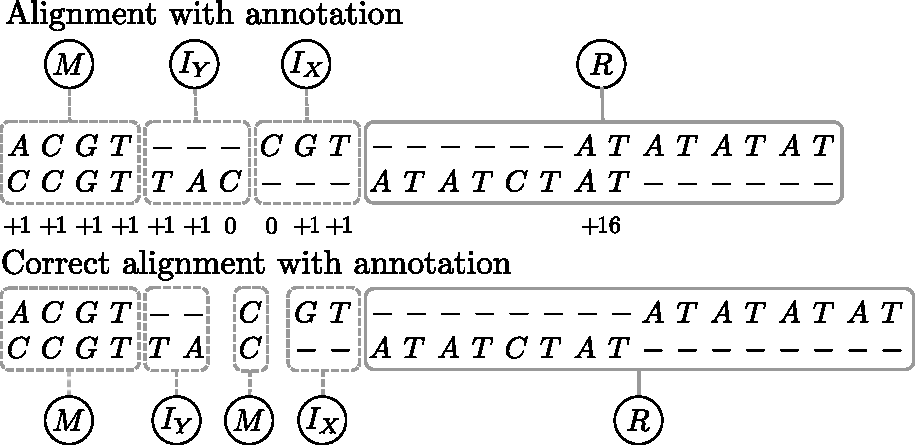
\includegraphics[width=11cm]{../figures/BlockPosterior.pdf}
\end{center}
\caption[Block posterior decoding function]{ 
An example of the BPD gain function. Gray solid boxes enclose single emissions,
dashed boxes combine multiple emissions (each alignment column in such a box is
one emission). Emission from repeat state have gain $+16$ because it emits $16$
sequences in exactly same regions of the input sequences.  Other alignment
columns get $+1$ only if there is same alignment column in the correct
alignment that was generated by same state.

}\label{FIGURE:BLOCK_POSTERIOR} 
\end{figure}

The reason for using score $+l$ instead of $+1$ is that otherwise the decoding method
would be biased towards short blocks. Instead of $l$, the number of emitted
symbols, we could use the number of emitted columns. However we would then
discriminate the submodels that would tried to align repeats (although we did
not used such models). An example of this gain function in Figure
\ref{FIGURE:BLOCK_POSTERIOR}.

To optimize this gain function, we have to compute posterior probabilities for
all potential emissions. In a generalized pHMM, each emission is given by a
state and two intervals; one in sequence $X$ and one in sequence $Y$. In our
models, only state $R$ is generalized and the overall number of states is
constant. The number of possible emissions is therefore $O(n^2m^2)$. The
expected gain of the emission is the posterior probability multiplied by the
number of emitted symbols. After computing the expected gains of individual blocks,
we can compute the highest scoring annotated alignment in $O(n^2m^2)$ time. \todo{Ako? aspon strucne}

Let $E$ be the number of transitions in the repeat submodel. The naive
\reformulate{computation}{detaily preco} of the expected gain for a pair of
intervals of length $n'$ and $m'$ can be computed in $O(n'm'E)$ time by the
forward algorithm for generalized pair HMMs, which would lead to $O(n^3m^3E)$
algorithm for computing all posterior probabilities by forward-backward
algorithm\todo{toto mam pocit ze ej aj tak zle}. We will show that by using
proper preprocessing  we can lower the time complexity of computing the
expected gain for a pair of intervals to $O(k)$ where $k$ is the number of
sunflower submodels (in case of TTP, $k=1$).

Let us consider the repeat submodel $H$ with $k$ sunflower pairs $S^X_1, S^Y_1,
\dots, S^X_k, S^Y_k$. Let $p_i$ be the probability of entering sunflower
$S^X_i$.  The probability of transition from $S^X_i$ to $S^Y_i$ is $1$. We can
write the probability of generating an arbitrary pair of sequences $X'$ and
$Y'$ by $H$ as

\begin{equation}
\prob{X', Y'\mid H} = \sum_{i=1}^k p_i\prob{X'\mid S^X_i}\prob{Y'\mid S^Y_i}
\end{equation}

By pre-computing all of the terms $\prob{X'\mid S^X_i}$ and $\prob{Y'\mid
S^Y_i}$, we can compute the posterior probability of the block in $O(k)$ time.
Naive computation of probability $\prob{X'\mid S^X_i}$ for all intervals $X'$
would take $O(n^3E)$ time, but this can be further improved. When computing
$\prob{X'\mid S^X_i}$ using the forward algorithm, we can use the values from
the forward table to compute the probability of emitting any prefix of $X'$ by
looking at the forward probability of final state for the corresponding column.
We thus need to run the forward algorithm only once for every suffix of $X$.
The optimization for the other sequence is analogous. Using these techniques,
we can pre-compute the emission terms in $O((n^2+m^2)E)$ time, and the overall
time complexity of the BPD is $O(kn^2m^2 + (n^2+m^2)E)$. \reformulate{By same
techniques we can optimize the BVA with same time complexity}{nejake detaily
cim sa lisy}.

\paragraph{Post-processing}
The problem with the SFF and the TTP models is that they model repeat sequences
in the sequences $X$ and $Y$ independently and do not try to align tandem
repeats at orthologous locations.  Therefore we postprocess the alignment using
the 3-state pHMM by realigning segments of alignments that are annotated as
repeats. We also include adjacent gaps into this postprocess step.

\section{Optimizations}\label{SECTION:REPOPT}

In this section, we summarize additional techniques we have used to decrease the
running time of the decoding algorithms. The fastest decoding algorithms described
above run in $O(nmE)$ time, which is still prohibitive for longer sequences.
Additionally, block-based methods are even slower. We used the following
optimizations:

\paragraph{}
We implemented a standard technique of banding (Section \ref{SECTION:SSA}). We
first align input sequences using Muscle \cite{Edgar2004} with default
parameters.  The final alignment methods were then restricted to be within 30
bases from this guide alignment. This technique reduces the $O(nm)$ factor from
the time complexity to $O((n+m)d)$ where $d$ is the maximum distance from the
guide alignment.

\paragraph{}
The size of the SFF model is enormous. It is not practical to use a model with
$310,091$ sunflower pairs. Therefore we used the TRF program \cite{Benson1999}
to find consensus motifs in the input alignment and used only those to build
SFF model. Note that the transition probabilities to individual sunflower pairs
were kept the same as in the original model. In case that TRF found a consensus
that was not in the original set of consensus sequences used to build the SFF
model, we assign it the probability of the least frequent consensus from the
original set. This technique is not applicable to TTP model.

\paragraph{}
To further reduce the running time of the block-based algorithms (BVA and BPD),
we restrict the emissions of the state $R$ to specific intervals in both input
sequences. First, we find the candidate set of tandem repeat intervals for
each input sequence independently. Let $T_X$ and $T_Y$ are the
sets of candidate intervals (not necessarily disjoint) for sequences $X$ and
$Y$ respectively. We restrict emission of state $R$ only to the pairs of
intervals $i_X, i_Y$ where $i_X$ and $i_Y$ have beginning and end within $10$
bases from some interval from $T_X$ and $T_Y$ respectively, or if one of $i_X$
or $i_Y$ is an empty interval (there can be a tandem repeat in only one
sequence).  By this heuristic, state $R$ can have emissions in at most
$(400|T_X|+n)(400|T_Y|+m)$ positions. We applied this method to both SFF and
TPP models.

We used the following algorithm to select candidate intervals $T_X$ and $T_Y$:
\begin{enumerate}[itemsep=-1mm]
\item Run the TRF program on the input sequences $X$ and $Y$. Obtain sets of
intervals $T_X$ and $T_Y$ and lists of consensus sequences $C_X$ and $C_Y$.

\item For every consensus $c\in C_X\cup C_Y$, build the SRF model $S_c$
(sunflower repeat finding model from Section \ref{SECTION:SUNFLOWERMODEL}). 

\item Each model $S_c$ is run on the sequences $X$ and $Y$ using the Viterbi
algorithm. All found repeat intervals are added into corresponding sets $T_X$
and $T_Y$.

\end{enumerate}
The reason for using this method instead of using only intervals from TRF is
that running TRF on the input sequences independently can cause several
problems. For example, if sequence $X$ contains three repetitions of motif $m$
and sequence $Y$ contains only one, then the TRF would return interval only for
sequence $X$. Additionally, consensus can be found in both sequences but can be
rotated, and therefore intervals in both sequences would be shifted.


\section{Experiments}
\todo{Dost hluba sekcie, daj to ako 2 subsections do experiments}

\todo{Poriadny uvod k experimentom,. Co ideme porovnavat s cim, a na akych datach. Preco a s nadhladom}

At first, we estimated parameters of the model
using annotated human-dog alignment by TRF program \cite{Benson1999}.
Parameters for 3-state model, and 3-state submodel of SFF and transitions to
the repeat state were therefore trained by supervised learning. Setting SFF and
TTP parameters was discussed in the sections \ref{SECTION:SUNFLOWERMODEL} and
\ref{SECTION:TANTAN}.\todo{tento odstavec Nejako pridaj do 4.2.2 a 4.2.3}
\subsection{Simulated data}
We sampled 200 test alignments each of length at least 200 bases from the SFF
submodel with the \reformulate{condition}{Ako sa realizovala tato [podmienka}, that the number of repetitions in the tandem
repeat has to be at least three in both sequences. Reason for this is that
otherwise we would have many segments of alignments that are annotated as repeats,
but in fact contain only one copy of the motif. We
refer to these alignments (along with the sampled repeat annotation) as the correct
alignments and correct annotation (repeat intervals and consensuses).  The
program Context \cite{Hickey2011} was trained of the 200 separate alignments
sampled from the model. 

\reformulate{
We used the same model for evaluation of parameters. To evaluate the robustness
of our method, we assess the effects of misspecification of the parameters by
estimating model parameters from human-chicken alignment and perturbing model
parameters (details are in the next section).}{Daj to len na jedno miest (zrejme az tam dalej)}

\paragraph{Accuracy measures} \todo{Uvod ze na porovnavanie spravnych zarovnani
a predikcii pouzivame niekolko mier}The first measure we used was the error
rate: the fraction of incorrectly predicted columns of an alignment. It was
measured only on the alignment columns generated from non-repeat states during
sampling, because SFF and TTP do not model alignment of
repetitive regions.

Additionally, we investigate the accuracy of predicting exact repeat block
boundaries in alignments by measuring the number of correctly predicted repeat
blocks; a block is correctly predicted if it contains identical parts of the
sequences as the corresponding block in the correct alignment. We report the
block sensitivity, which is the number of correctly predicted blocks divided by
the number of all repeat blocks in the correct alignment, and block
specificity, which is the the number of correctly predicted blocks divided by
the number of all predicted blocks.  We also investigate the accuracy of
prediction of repeat annotation for individual \reformulate{alignment
columns}{je to na stlpce alebo bazy}; the repeat sensitivity and specificity.

\reformulate{We also measured the relation of the error rate and the distance
from the nearest repeat. Alignment column was considered as repeat if in the
correct alignment at least one base of the column was annotated as an repeat.
The distance is measured by the number of columns. This measure is important,
because when the distance from the repeat is high, our model is identical to
3-state pHMM and therefore the performance of both models should be similar in
such regions. However, we do expect models incorporating repeats to be more
precise in the regions near tandem repeats.}{presun k vysledkom}

\section{Results of the Simulation Experiments}\label{SECTION:REPSIMRESULTS}

This section discuss the results of the simulation experiment. We split results
of various version of algorithms into several tables. The results for SFF and
TTP models are in the Table \ref{TABLE:SFFMAIN}. Table
\ref{TABLE:SFFMAINORIGINAL} contain results for same algorithms, but with use
of the correct intervals and motifs instead of of their approximations obtained
by TRF program. Results for the non-SFF alignment programs and methods for
aligning sequences with repeats is in the Table \ref{TABLE:SFFOTHER}. The
effects of misspecification of mode parameters is in the Table
\ref{TABLE:SFFMARGINALIZED} and the effects of different masking methods on
posterior and Viterbi algorithm is in the table \ref{TABLE:SFF3STATEMASK}.
Figure \ref{FIGURE:SFF_GRAPHS} compare the relation between the error rate and
the distance from the repeat for studied methods. Following text contain the
discussion of the results.

\def\M{$^\circ$} % mark by a star
\def\MM{$^{\circ\circ\circ}$} % mark by two stars
\def\D{$^{\circ\circ}$} % mark by dagger
\def\DD{$^{\dagger}$} % mark by dagger
\def\R{$^{\yen}$}
\def\RR{$^{\yen\yen}$}
\def\CC#1{\multicolumn{1}{c}{#1}} % center column
\def\S{$^{\star}$}

\begin{table*}
\begin{center}
\begin{tabular}{lr@{\quad}rr@{\quad}rr}
\hline
          & \CC{Alignment} & \multicolumn{2}{c}{Repeat} & 
\multicolumn{2}{c}{Block}\\
Algorithm & \CC{error} & \CC{sn.} & \CC{sp.} & \CC{sn.} & \CC{sp.} \\
\hline
\hline
%\hline
3-state VA (baseline)    & 4.78\% \\
\hline
SFF MPD   & {\bf 3.37\%} & {\bf 95.97\%} & 97.78\% & {\bf 43.07\%} & 44.87\%\\
SFF PD    & 3.53\% & 95.86\% & 97.87\% & 42.70\% & 47.37\%\\
SFF BPD   & 3.51\% & 93.09\% & {\bf 98.07}\% & 36.50\% & 41.67\%\\
SFF BVA   & 3.91\% & 93.26\% & 97.96\% & 35.77\% & 40.66\%\\
SFF VA    & 4.04\% & 95.29\% & 97.85\% & 42.70\% & {\bf 48.95\%}\\
TANTAN BPD& 5.05\% & 61.38\% & 97.48\% & 0.00\% & 0.00\%\\
TANTAN BVA& 6.17\% & 67.86\% & 96.51\% & 0.00\% & 0.00\%\\
\hline
\end{tabular}
\end{center}
\caption{Accuracy of decoding methods on simulated data.}\label{TABLE:SFFMAIN}
\end{table*}

Since we run the decoding algorithms described in the section
\ref{SECTION:REPDECODING} with various combination of additional information
(i.e. repeat intervals and motifs), we use following symbols to
distinguish them.

\begin{itemize}[itemsep=-1mm]

\item[\M] method uses the correct motifs. 

\item[\D] method uses intervals from the correct repeat blocks.

\item[\MM] method uses the correct motifs and intervals from the
correct repeat blocks.

\item[\R] Parameters of the three-state submodel were estimated from
human-chicken alignment. 

\item[\RR] Parameters of SFF submodel were perturbed randomly.

\item[\DD] Columns with at least one masked character are considered as
repeats.

\item[\S] Non-overlapping set of repeats from TRF output with maximal total
score is used.

\end{itemize}

In general, using SFF model decreased the alignment error rate by $15-30\%$ as
opposed to baseline method as can be seen in table \ref{TABLE:SFFMAIN}. The
$15\%$ decrease was obtained by replacing 3-state model with the Sunflower Field
model, other improvements were through using different decoding algorithms,
with the marginalized posterior decoding having the lowest error rate. The
Viterbi based methods had consistently higher error rate than posterior based
methods and the block-based versions of the algorithms decreased the error rate
by at most $3.3\%$ as opposed to non-block based methods. Surprisingly, block
based methods had poorest performance in the block sensitivity and specificity
and repeat sensitivity. These measures are closer to what block methods
optimize, so we expected opposite. Reason for this is perhaps due to
approximate {intervals and/or motifs obtained TRF and SRF}, since when running
algorithms that uses correct intervals and motifs (see Table
\ref{TABLE:SFFMAINORIGINAL}), their performance improved significantly.
Results in Table \ref{TABLE:SFFMAINORIGINAL} helps us to quantify the effect of
not using the exact repeat intervals and also can be used as an upper bounds
for the performance of our models. There is clearly room for improvements of
repeat intervals, we could perhaps try to use other programs that detect tandem
repeats, like ATRhunter \cite{Wexler2005} or mreps \cite{Kolpakov2003}.

\begin{table*}
\begin{center}
\begin{tabular}{lr@{\quad}rr@{\quad}rr}
\hline
          & \CC{Alignment} & \multicolumn{2}{c}{Repeat} & 
\multicolumn{2}{c}{Block}\\
Algorithm & \CC{error} & \CC{sn.} & \CC{sp.} & \CC{sn.} & \CC{sp.} \\
\hline
\hline
%\hline
3-state VA (baseline)    & 4.78\% \\
\hline
SFF MPD\M            & {\bf 3.02}\% & {\bf 98.93}\% & 99.64\% & 77.01\% & 76.17\% \\ 
SFF PD\M             & 3.42\% & 98.84\% & 99.51\% & 75.91\% & 80.93\% \\
SFF BPD\MM           & 3.21\% & 97.70\% & 99.87\% & 80.66\% & {\bf 94.44}\% \\
SFF BVA\MM           & 3.71\% & 98.12\% & 99.85\% & {\bf 81.75}\% & 92.18\% \\
SFF VA\M             & 3.94\% & 98.54\% & 99.45\% & 75.55\% & 83.47\% \\
TANTAN BPD\D         & 3.42\% & 60.45\% & {\bf 99.90}\% & 0.36\% & 0.46\% \\
TANTAN BVA\D         & 3.83\% & 61.74\% & 99.88\% & 0.00\% & 0.00\% \\
\hline
\end{tabular}
\end{center}
\caption{Accuracy of decoding methods using real motif and/or real intervals on simulated data.}\label{TABLE:SFFMAINORIGINAL}
\end{table*}

Similar behaviour was obtained for TTP model; using the original intervals, TTP
model has only slightly worse error rate than the SFF, which is expectable, since
the data were generated from the SFF model. However, using TRF for intervals,
TTP has significantly higher error rate, which means that TTP is even more
sensitive to the intervals that are used. Also the high error rate and low
repeat and block prediction performance could be caused by improperly treating
the first repetition, because annotations of TTP methods almost always skip the
first copy of repeat motif. Additionally, in TPP the motifs in tandem repeat
are not dependent between sequences, which can be also source of higher error
rate.  This could be improved by merging the chain of prefix states $P_1,
\dots, P_K$ into chain of match states aligning the first repetition.

Results of other alignment methods are in the Table \ref{TABLE:SFFOTHER}.
Namely the Context program, Muscle, 3-state posterior algorithm and 3-state
posterior algorithm with hard-masking. Apart from the 3-state posterior
algorithm, all methods had higher error rate than the baseline method. The high
error rate of the Context program could be caused by insufficient training data
or some software issues. We run muscle with default parameters and therefore
its scoring scheme was not tailored to our method. Using the hard-masking
produced alignment with higher error rate. It might be cause by the
insufficient accuracy of the tandem repeat annotation.

\begin{table*}
\begin{center}
\begin{tabular}{lr@{\quad}rr@{\quad}rr}
\hline
          & \CC{Alignment} & \multicolumn{2}{c}{Repeat} & 
\multicolumn{2}{c}{Block}\\
Algorithm & \CC{error} & \CC{sn.} & \CC{sp.} & \CC{sn.} & \CC{sp.} \\
\hline
\hline
%\hline
3-state VA (baseline)    & {4.78}\% \\
\hline
Context             & 5.98\% \\
Muscle              & 5.62\% \\
3-state PD   & \bf 4.41\% \\
3-state masked PD\DD & 5.03\% & 99.23\% & 74.16\% & 7.66\% & 7.24\%\\
\hline
\end{tabular}
\end{center}
\caption{Accuracy for standard algorithms and other tools on the simulated data.
Most of the methods did not annotate the alignment with tandem repeats and
therefore relating metrics are not available.
}\label{TABLE:SFFOTHER}
\end{table*}

Since we did use the same model for generating data and testing, we tried to
quantify the effect of misspecification of the model parameters.  SFF model
have two principal types of parameters; parameters of the 3-state HMM and
parameters of the Sunflower model. We investigate the effect of
{misspecification} for both types independently. For the parameters of 3-state
model, we have estimate the parameters from human-chicken alignments instead of
human-dog alignment. For the second type, we have perturbed the each parameter
of Sunflower model randomly by additive term from $0.02$ to $0.05$. On these
models we run marginalized posterior decoding. Table
\ref{TABLE:SFFMARGINALIZED} shows that our method is quite robust. Our method
is more sensitive to change in the training alignment, since the error rate for
MPD increased by $8\%$, but it is still significantly better than the baseline
method. Perturbing parameters for Sunflower submodel did not have significant
effect on error rate (increase by $0.5\%$). 

\begin{table*}
\begin{center}
\begin{tabular}{lr@{\quad}rr@{\quad}rr}
\hline
          & \CC{Alignment} & \multicolumn{2}{c}{Repeat} & 
\multicolumn{2}{c}{Block}\\
Algorithm & \CC{error} & \CC{sn.} & \CC{sp.} & \CC{sn.} & \CC{sp.} \\
\hline
\hline
%\hline
3-state VA (baseline)    & 4.78\% \\
\hline
SFF MPD    & 3.37\% & 95.97\% & 97.78\% & {\bf 43.07\%} & {\bf 44.87}\%\\
SFF MPD\R & 3.63\% & {\bf 96.03\%} & 97.74\% &  42.70\% &  43.33\% \\ 
SFF MPD\RR & {\bf 3.36}\% & 95.99\% & {\bf 97.81}\% & 40.88\% & 43.08\% \\ 
SFF MPD\M  & \bf 3.02\% & \bf 98.93\% & \bf 99.64\% &\bf 77.01\% &\bf 76.17\% \\ 
\hline
\end{tabular}
\end{center}
\caption{Accuracy for marginalized posterior decoding with different models or real motifs.
The best and the second best are bold.} \label{TABLE:SFFMARGINALIZED}
\end{table*}

Table \ref{TABLE:SFF3STATEMASK} investigates the use of the different repeat
finding methods for masking. We used the Sunflower model (modified for finding
tandem repeats as described in section \ref{SECTION:SUNFLOWERMODEL}), TRF, and
TRF with non-overlapping repeats (we select maximal scoring non-overlapping set
of tandem repeats out of TRF output). We used hard-masking as described in
section \ref{SECTION:REPALNMETHODS}. For decoding we used both the VA and the
PD.  Apart from  using correct intervals, the best performing masking was used
with non-overlapping repeats from TRF.

\begin{table*}
\begin{center}
\begin{tabular}{lr@{\quad}rr@{\quad}rr}
\hline
          & \CC{Alignment} & \multicolumn{2}{c}{Repeat} & 
\multicolumn{2}{c}{Block}\\
Algorithm & \CC{error} & \CC{sn.} & \CC{sp.} & \CC{sn.} & \CC{sp.} \\
\hline
\hline
%\hline
3-state Viterbi (baseline)    & 4.78\% \\
\hline
3 state masked PD, TRF\DD       &5.03&{\bf 99.23}&74.16&7.66&7.24\\
3 state masked PD, Sunflower\DD &5.21&98.30&68.65&{\bf 9.12}&7.53\\
3 state masked PD, TRF\S\DD     &{\bf 4.77}&88.17&{\bf 79.63}&7.66&{\bf 9.13}\\
3 state masked PD, \MM\DD       &{\bf 4.50}&{\bf 100.00}&{\bf 97.23}&{\bf 45.99}&{\bf 61.13}\\
\hline
3 state masked VA, TRF\DD         &5.89&{\bf 99.25}&73.29&5.47&5.14\\
3 state masked VA, Sunflower\DD   &5.82&98.32&67.90&{\bf 5.84}&4.89\\
3 state masked VA, TRF\S\DD       &{\bf 5.10}&88.33&{\bf 78.68}&5.47&{\bf 6.47}\\
3 state masked VA, \MM\DD         &{\bf 5.02}&{\bf 100.00}&{\bf 95.41}&{\bf 45.99}&{\bf 44.21}\\
\hline
\end{tabular}
\end{center}
\caption{Accuracy of decoding method using simple 3-state HMM and hard-masking. The best and the second best are bold. }\label{TABLE:SFF3STATEMASK}
\end{table*}

Finally, we investigate the relation between the error rate and the distance
from the nearest repeat. Figure \ref{FIGURE:SFF_GRAPHS} contains graphs for
this metric for various combination of parameters. In general, all algorithms
have highest error rate near boundaries of the repeat, with the error rate lowering
with the distance from the repeat. Most methods reach the baseline error rate
within distance $10$ bases of the repeat border.

\begin{figure}
\begin{center}
\begin{subfigure}{0.5\textwidth}
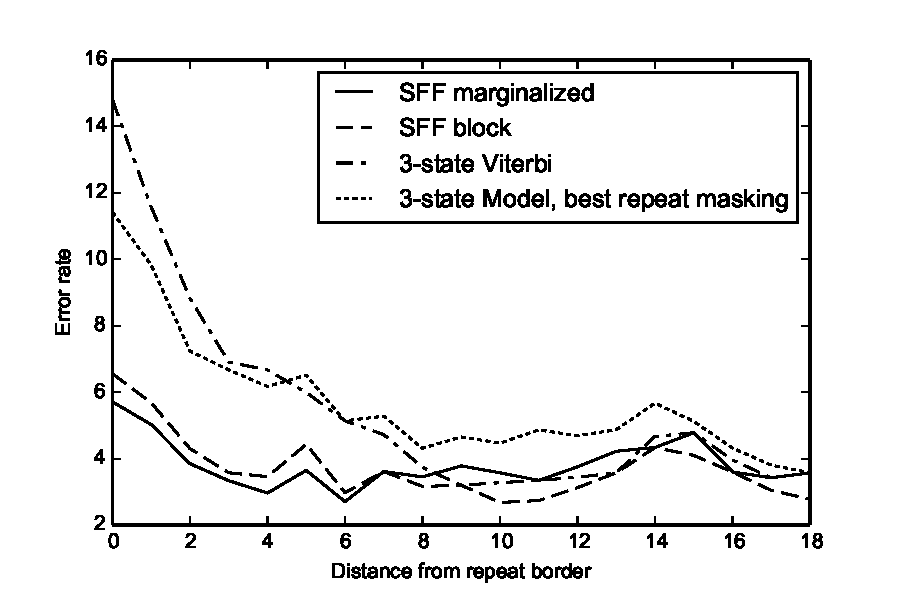
\includegraphics[width=\textwidth]{../figures/error_graph_overview.pdf}
\caption{Our methods and traditional methods}\label{FIGURE:SFFOVER}
\end{subfigure}%
\begin{subfigure}{0.5\textwidth}
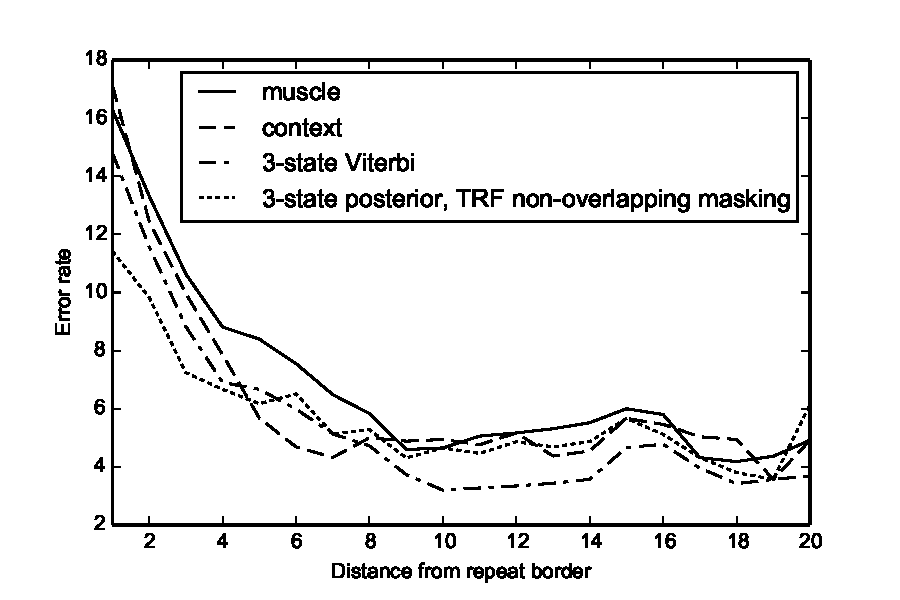
\includegraphics[width=\textwidth]{../figures/error_graph_other.pdf}
\caption{Other methods}\label{FIGURE:SFFOTHER}
\end{subfigure}%

\begin{subfigure}{0.5\textwidth}
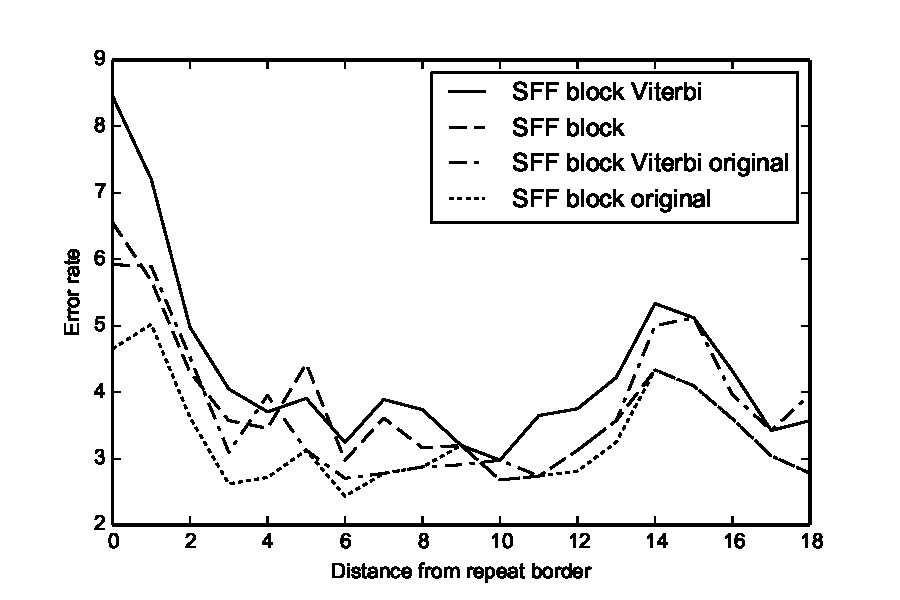
\includegraphics[width=\textwidth]{../figures/error_graph_sffblock.pdf}
\caption{Block decodings}\label{FIGURE:SFFBLOCKS}
\end{subfigure}%
\begin{subfigure}{0.5\textwidth}
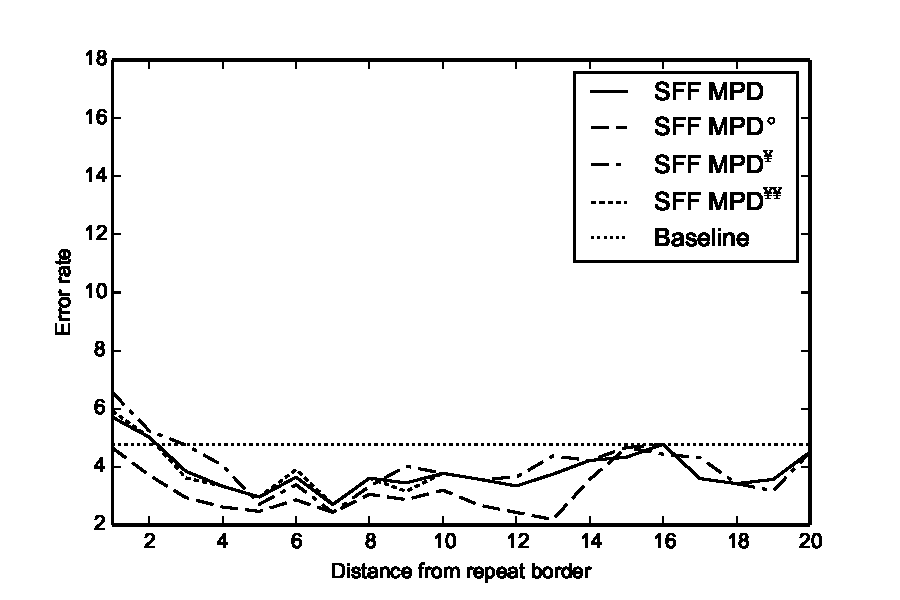
\includegraphics[width=\textwidth]{../figures/error_graph_marginalized.pdf}
\caption{Same method, different models}\label{FIGURE:SFFWEIRD}
\end{subfigure}%

\begin{subfigure}{0.5\textwidth}
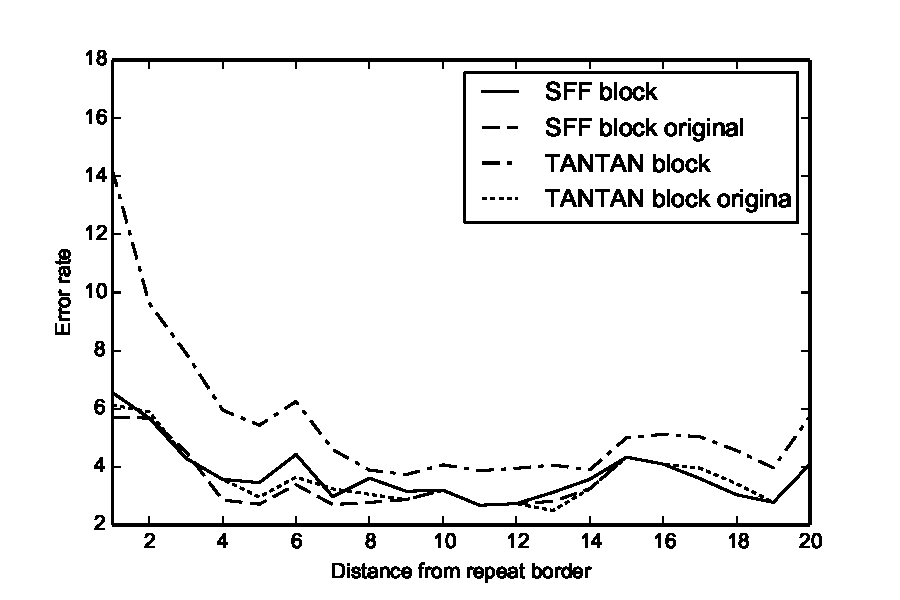
\includegraphics[width=\textwidth]{../figures/error_graph_sffvstantan.pdf}
\caption{Sunflower and TANTAN}\label{FIGURE:SFFTANTAN}
\end{subfigure}%
\begin{subfigure}{0.5\textwidth}
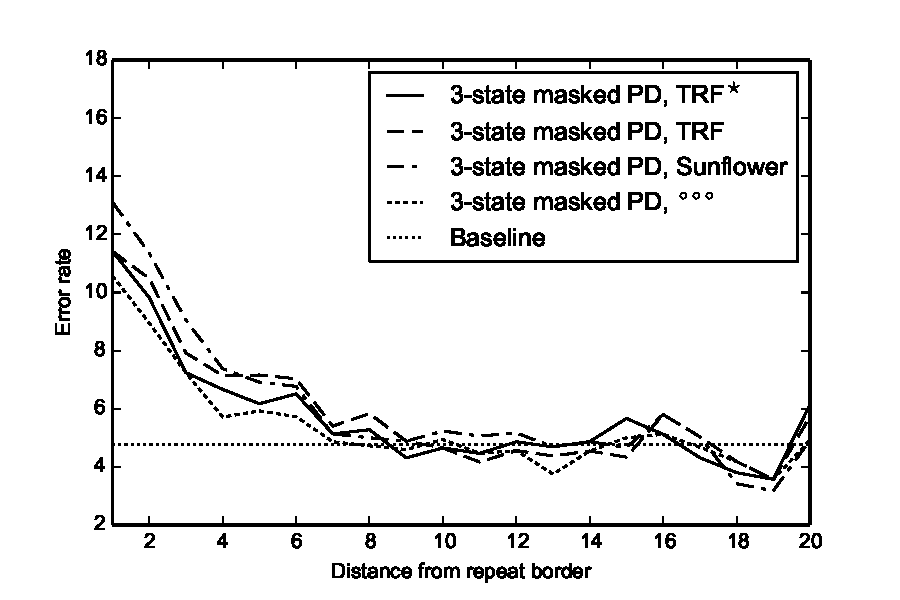
\includegraphics[width=\textwidth]{../figures/error_graph_3statemasking.pdf}
\caption{Different methods of masking}
\end{subfigure}%
\caption{
The relation between the error rate and the distance from the nearest repeat. On the Y
axis is error rate of the algorithm; the number of incorrectly aligned columns.
On the X axis is the distance from the nearest repeat. Baseline is the overall
error rate, with no relation to the distance from the repeat border, for
3-state model with the VA.
}\label{FIGURE:SFF_GRAPHS} 
\end{center}
\end{figure}

Figures \ref{FIGURE:SFFOVER} and \ref{FIGURE:SFFOTHER} suggests that the right
selection of decoding method can improve error rate near repeats, but most of
the drop in the error rate was caused by using SFF model. As with other
metrics, TTP with correct intervals performs similarly to SFF model, but TTPs
error rate near repeats raises significantly where intervals were obtained from
TRF (see Figure \ref{FIGURE:SFFTANTAN}). Using different  model did not have
large effect also on the error rate as we can see in the Figure
\ref{FIGURE:SFFWEIRD}. Figure \ref{FIGURE:SFFBLOCKS} demonstrates that for
block methods, using block Viterbi double the error rate near repeat.


\begin{comment}
\section{Possible Improvements}

\begin{reformulate*}
Sem by som mohol napisat, ako by sa dal pouzit symetricky model s cyklom
stavov, alebo ako by sa dal ten cyklus stavov odstranit odstranenim jednej
hrany a pridanych n hran -- co je lepsie ako pridat n vrcholov.
\end{reformulate*}
\end{comment}
